\documentclass[12pt]{beamer}
\usepackage[utf8]{inputenc}
\usepackage[T1]{fontenc}
\usepackage[portuguese]{babel} % Alterado de espanhol para português
\usepackage{xcolor}
\usepackage{tcolorbox}
\usepackage{amsthm}
\usepackage{amsmath}
\usepackage{lipsum}
\usepackage{tikz}
\usepackage{lmodern}
\usepackage{graphicx}
\usepackage[boxed,algoruled,linesnumbered]{algorithm2e}
\renewcommand{\familydefault}{\sfdefault}


% Configuração de algorithm2e para Beamer
\SetAlgoNlRelativeSize{-1}
\SetNlSty{textbf}{(}{)}
\SetAlFnt{\small}
\SetInd{0.5em}{0.5em} % Ajusta a indentação
\SetAlCapSkip{1em}

% ====== DEFINIÇÃO DE CORES ======
\definecolor{rojoUNI}{HTML}{D16969}
\definecolor{doradoUNI}{HTML}{DBCB9F}
\definecolor{rojoSuave}{HTML}{d39c9c}
\definecolor{doradoClaro}{HTML}{eee5cd}
\definecolor{grisNeutro}{HTML}{9B9B9B}

% ====== CONFIGURAÇÃO BEAMER ======
%\usetheme{Madrid}
%\usecolortheme{default}

% Personalização de cores do Beamer
\setbeamercolor{title}{fg=rojoUNI}
\setbeamercolor{frametitle}{fg=rojoUNI}
\setbeamercolor{structure}{fg=rojoUNI}
\setbeamercolor{normal text}{fg=black}
\setbeamercolor{block title}{fg=white, bg=rojoUNI}
\setbeamercolor{block body}{fg=black, bg=doradoClaro!40}

% Rodapé personalizado
\setbeamertemplate{footline}{
  \begin{tikzpicture}[remember picture,overlay]
    \node at (current page.south) [anchor=south, yshift=0.6cm] {
      
\includegraphics[width=0.85\paperwidth,height=0.8cm]{img/footage-red.pdf}
    };
  \end{tikzpicture}
  \hspace*{0.1\paperwidth}
  \raisebox{0.5cm}[0pt][0pt]{
    \color{rojoUNI}\bfseries\insertshorttitle
  }
  \hfill
  \raisebox{0.5cm}[0pt][0pt]{
    \color{rojoUNI}\bfseries\insertframenumber/\inserttotalframenumber
  }
  \hspace*{0.1\paperwidth}
}

% Configuração de blocos
\newtcolorbox{definicao}[1][]{colback=doradoClaro!40,
  colframe=rojoUNI, fonttitle=\bfseries\color{white},
  title=Definição, #1}

\newtcolorbox{teorema}[1][]{colback=white,
  colframe=doradoUNI, fonttitle=\bfseries\color{black},
  title=Teorema, #1}

\newtcolorbox{lema}[1][]{colback=white,
  colframe=rojoSuave, fonttitle=\bfseries\color{white},
  title=Lema, #1}

\newtcolorbox{exemplo}[1][]{colback=white,
  colframe=rojoSuave!80!black, fonttitle=\bfseries\color{white},
  title=Exemplo, #1}

\newtcolorbox{restricao}[1][]{colback=doradoClaro,
  colframe=grisNeutro, fonttitle=\bfseries\color{white},
  title=Restrição, #1}

\newtcolorbox{restricoesPC}[1][]{colback=doradoClaro!40,
  colframe=rojoUNI, fonttitle=\bfseries\color{white},
  title=Restrições, #1}

\newtcolorbox{bloco}[1][]{
  colback=doradoClaro!40,
  colframe=rojoUNI,
  fonttitle=\bfseries\color{white},
  title=#1}

% ====== DOCUMENTO ======
\title{Greedy para zebras}
\author{Miguel Miní}
\date{2025}

\begin{document}

\begin{frame}

  {\hspace{9cm}
\includegraphics[width=0.15\textwidth]{img/unicamp.png}}
  
  %\vspace{-0.5cm}
  
  % Título
  
  {\hspace{0.5cm}\bfseries\Huge \textcolor{rojoUNI}{Greedy para zebras}}

   \vspace{0.5cm}
  {\hspace{0.6cm}\textcolor{rojoUNI}{Miguel Miní}}
  
  \vfill
\end{frame}


\begin{frame}{Árvore de Huffman}

\begin{definicao}
    A Árvore de Huffman de uma sequência $\{w_1, w_2, \dots, w_n\}$ é uma árvore binária com $n$ folhas, que minimiza

\[
    \sum_{i=1}^n w_i \times d_i  
\]

    Onde $d_i$ ($1 \le i \le n$), é a profundidade da i-ésima folha na árvore.
\end{definicao}
  
\end{frame}

\begin{frame}

\begin{exemplo}
\begin{columns}
\begin{column}{0.6\textwidth}
Árvore de Huffman com custo 
\begin{align*}
    &w_1 \times 2 + w_2 \times 2 + w_3 \times 1\\
    &2 \times 2 + 3 \times 2 + 6 \times 1 = 16
\end{align*}

\textbf{Nota:} Também podemos comprimir frases usando o caminho para cada letra (esquerda: 0, direita: 1).
    
\end{column}

\begin{column}{0.31\textwidth}
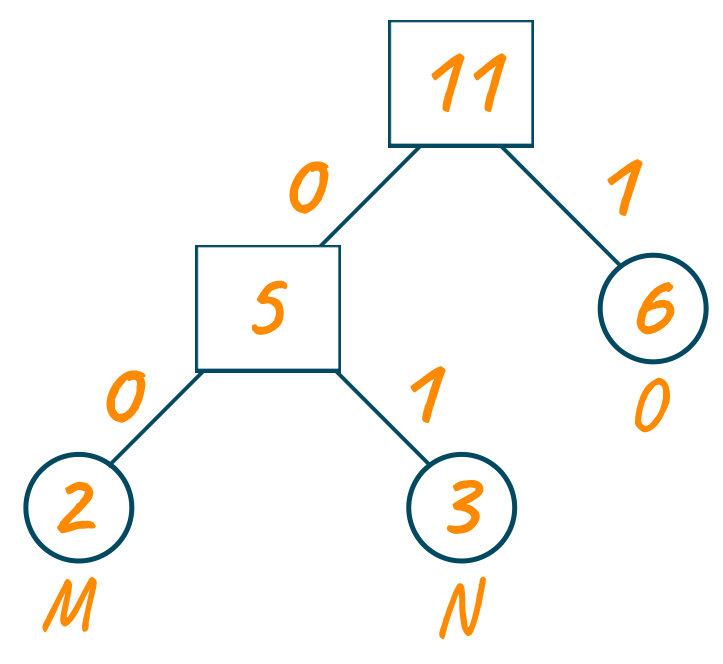
\includegraphics[width=\textwidth]{img/huffman.png}    
\end{column}

\end{columns}
\end{exemplo}

\end{frame}

\begin{frame}
\hspace*{0.5cm} % Ajuste para mover o algoritmo para a direita
\begin{minipage}{0.93\textwidth}
\SetAlFnt{\footnotesize} % Reduzir tamanho da fonte
\begin{algorithm}[H]
  \KwIn{sequência $w_1, w_2, \dots, w_n$}
  \KwOut{Árvore de Huffman}
  min heap $Q$ com todas as folhas ($nodo_i, w_i$), ordenados por $w_i$\;
  \While{$|Q| > 1$}{
      $(node_i, w_i)\leftarrow$ extrair topo de $Q$\;
      $(node_j, w_j) \leftarrow$ extrair topo de $Q$\;
      Criar um novo nó $node_z$ com filhos $node_i$ e $node_j$\;
      Atribuir $w_z = w_i + w_j$\;
      Inserir $(node_z, w_z)$ na fila $Q$\;
  }
  \Return{O único nó restante em $Q$ (raiz da árvore)}
  \caption{Construção de uma Árvore de Huffman}
\end{algorithm}
\end{minipage}
\end{frame}

\begin{frame}
\begin{exemplo}
\begin{figure}
    \centering
    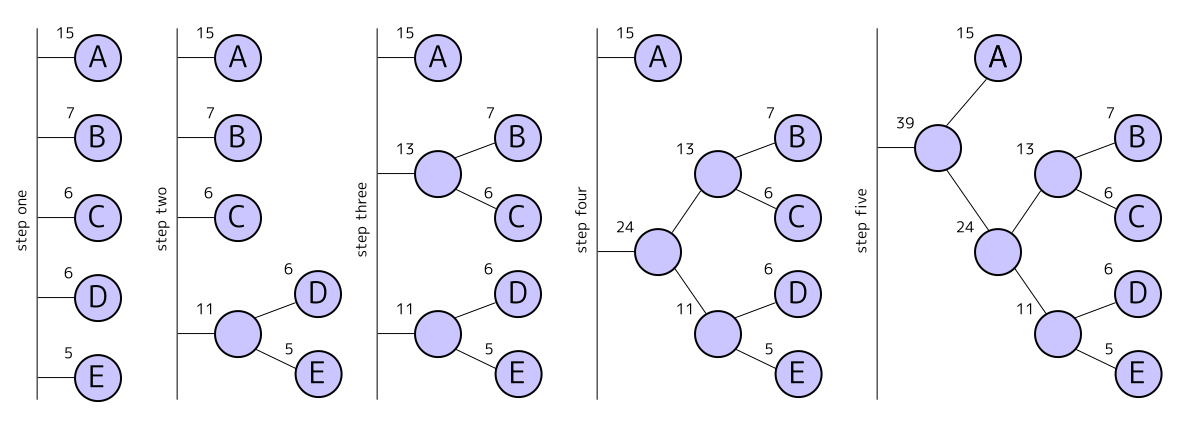
\includegraphics[width=1\linewidth]{img/huffmanalgorithm.png}
    \label{fig:enter-label}
\end{figure}  
\end{exemplo}    
\end{frame}

\begin{frame}
\begin{bloco}[Revisitando a Árvore de Huffman]
Dado que o algoritmo é ótimo*, podemos concluir que este tem um custo inferior a alguma configuração, assim:

\[
\sum_{i=1}^n w_i \times d_i \le \left(\sum_{i=1}^n w_i\right) \log (n)
\]

\pause

\textbf{dica:}

\begin{figure}
    \centering
    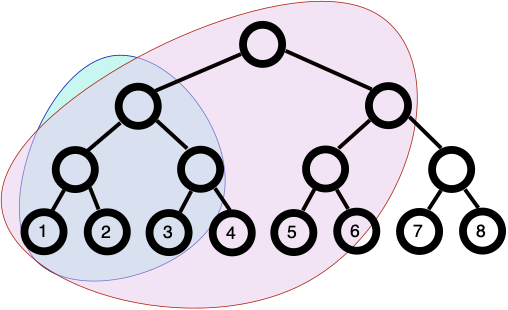
\includegraphics[width=0.4\linewidth, height=0.23\textwidth]{img/complete.png}
    \label{fig:enter-label}
\end{figure}

\end{bloco}
\end{frame}

\begin{frame}
\begin{bloco}[Revisitando a Árvore de Huffman]

Sejam $n$ conjuntos com pesos $\{w_1, w_2, \dots, w_n\}$, e devemos formar um conjunto que contenha todos eles, tal que:

\begin{itemize}
    \item escolhemos dois conjuntos $s_x$ e $s_y$.
    \item criamos um novo conjunto $s_z = s_x \cup s_y$, com custo $w_z = w_x + w_y$.
    \item substituímos $s_x$ e $s_y$ por $s_z$.
\end{itemize}

Desejamos que a soma dos custos seja mínima.

\end{bloco}
\end{frame}

\begin{frame}
\begin{bloco}[Revisitando a Árvore de Huffman]
O problema é equivalente a encontrar uma Árvore de Huffman?

\begin{columns}
\begin{column}{0.4\textwidth}
\begin{figure}
    \centering
    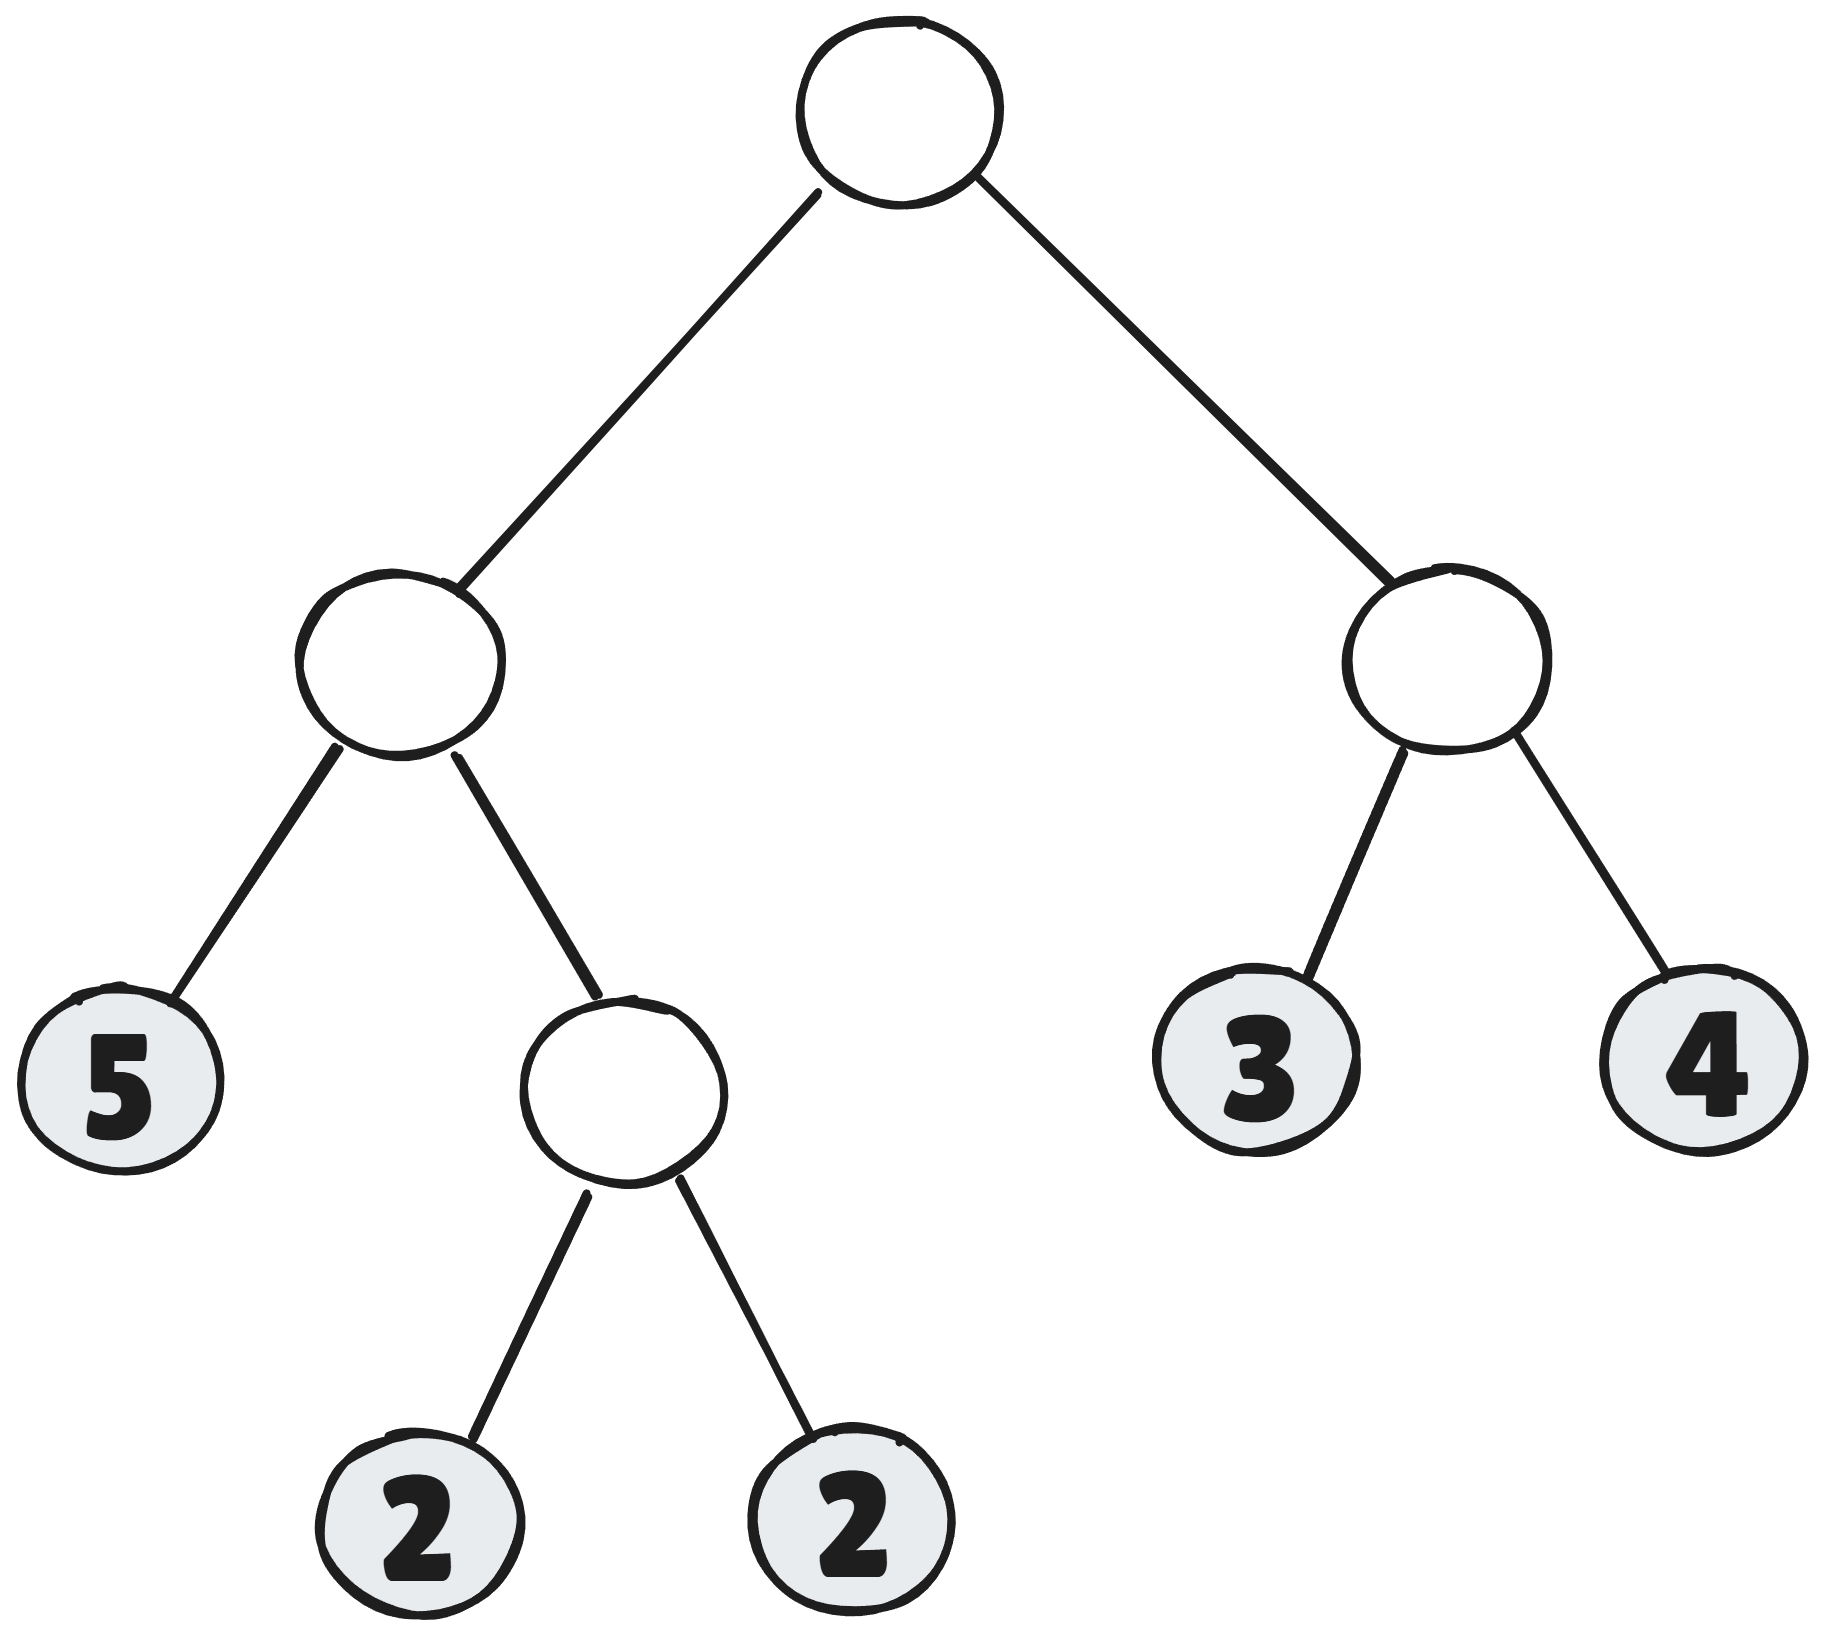
\includegraphics[width=\linewidth]{img/ht1.png}
    \label{fig:enter-label}
\end{figure}
\end{column}
\begin{column}{0.4\textwidth}
\begin{figure}
    \centering
    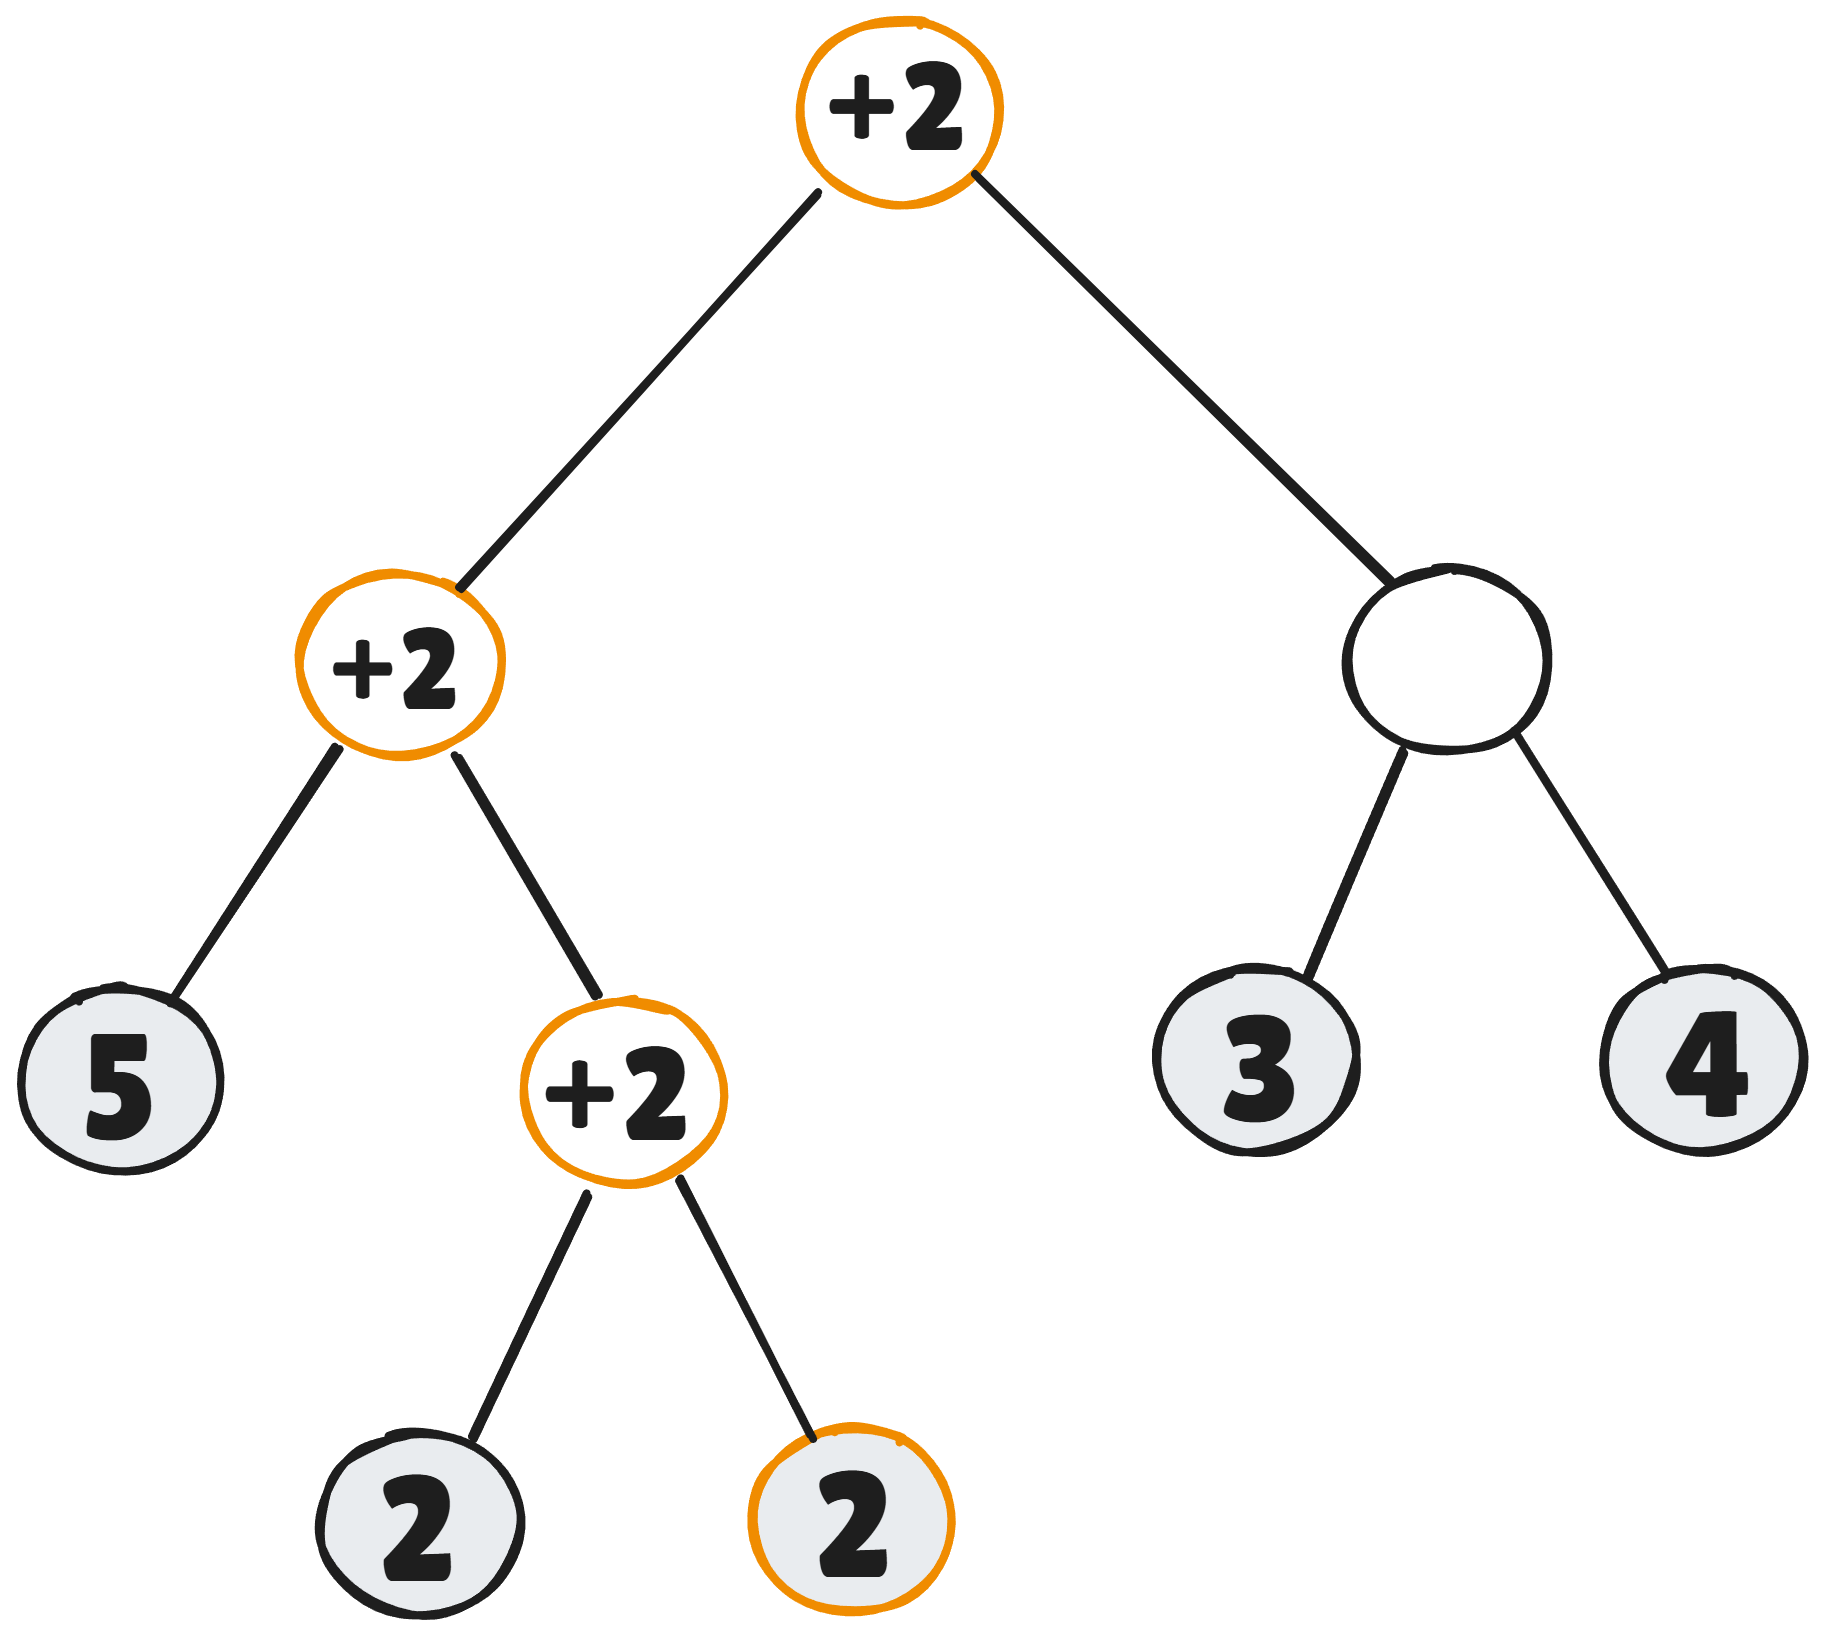
\includegraphics[width=\linewidth]{img/ht2.png}
    \label{fig:enter-label}
\end{figure}
\end{column}
\end{columns}
\end{bloco}
\end{frame}

\begin{frame}
\begin{bloco}[Revisitando a Árvore de Huffman]
O problema é equivalente a encontrar uma Árvore de Huffman?

\begin{figure}
    \centering
    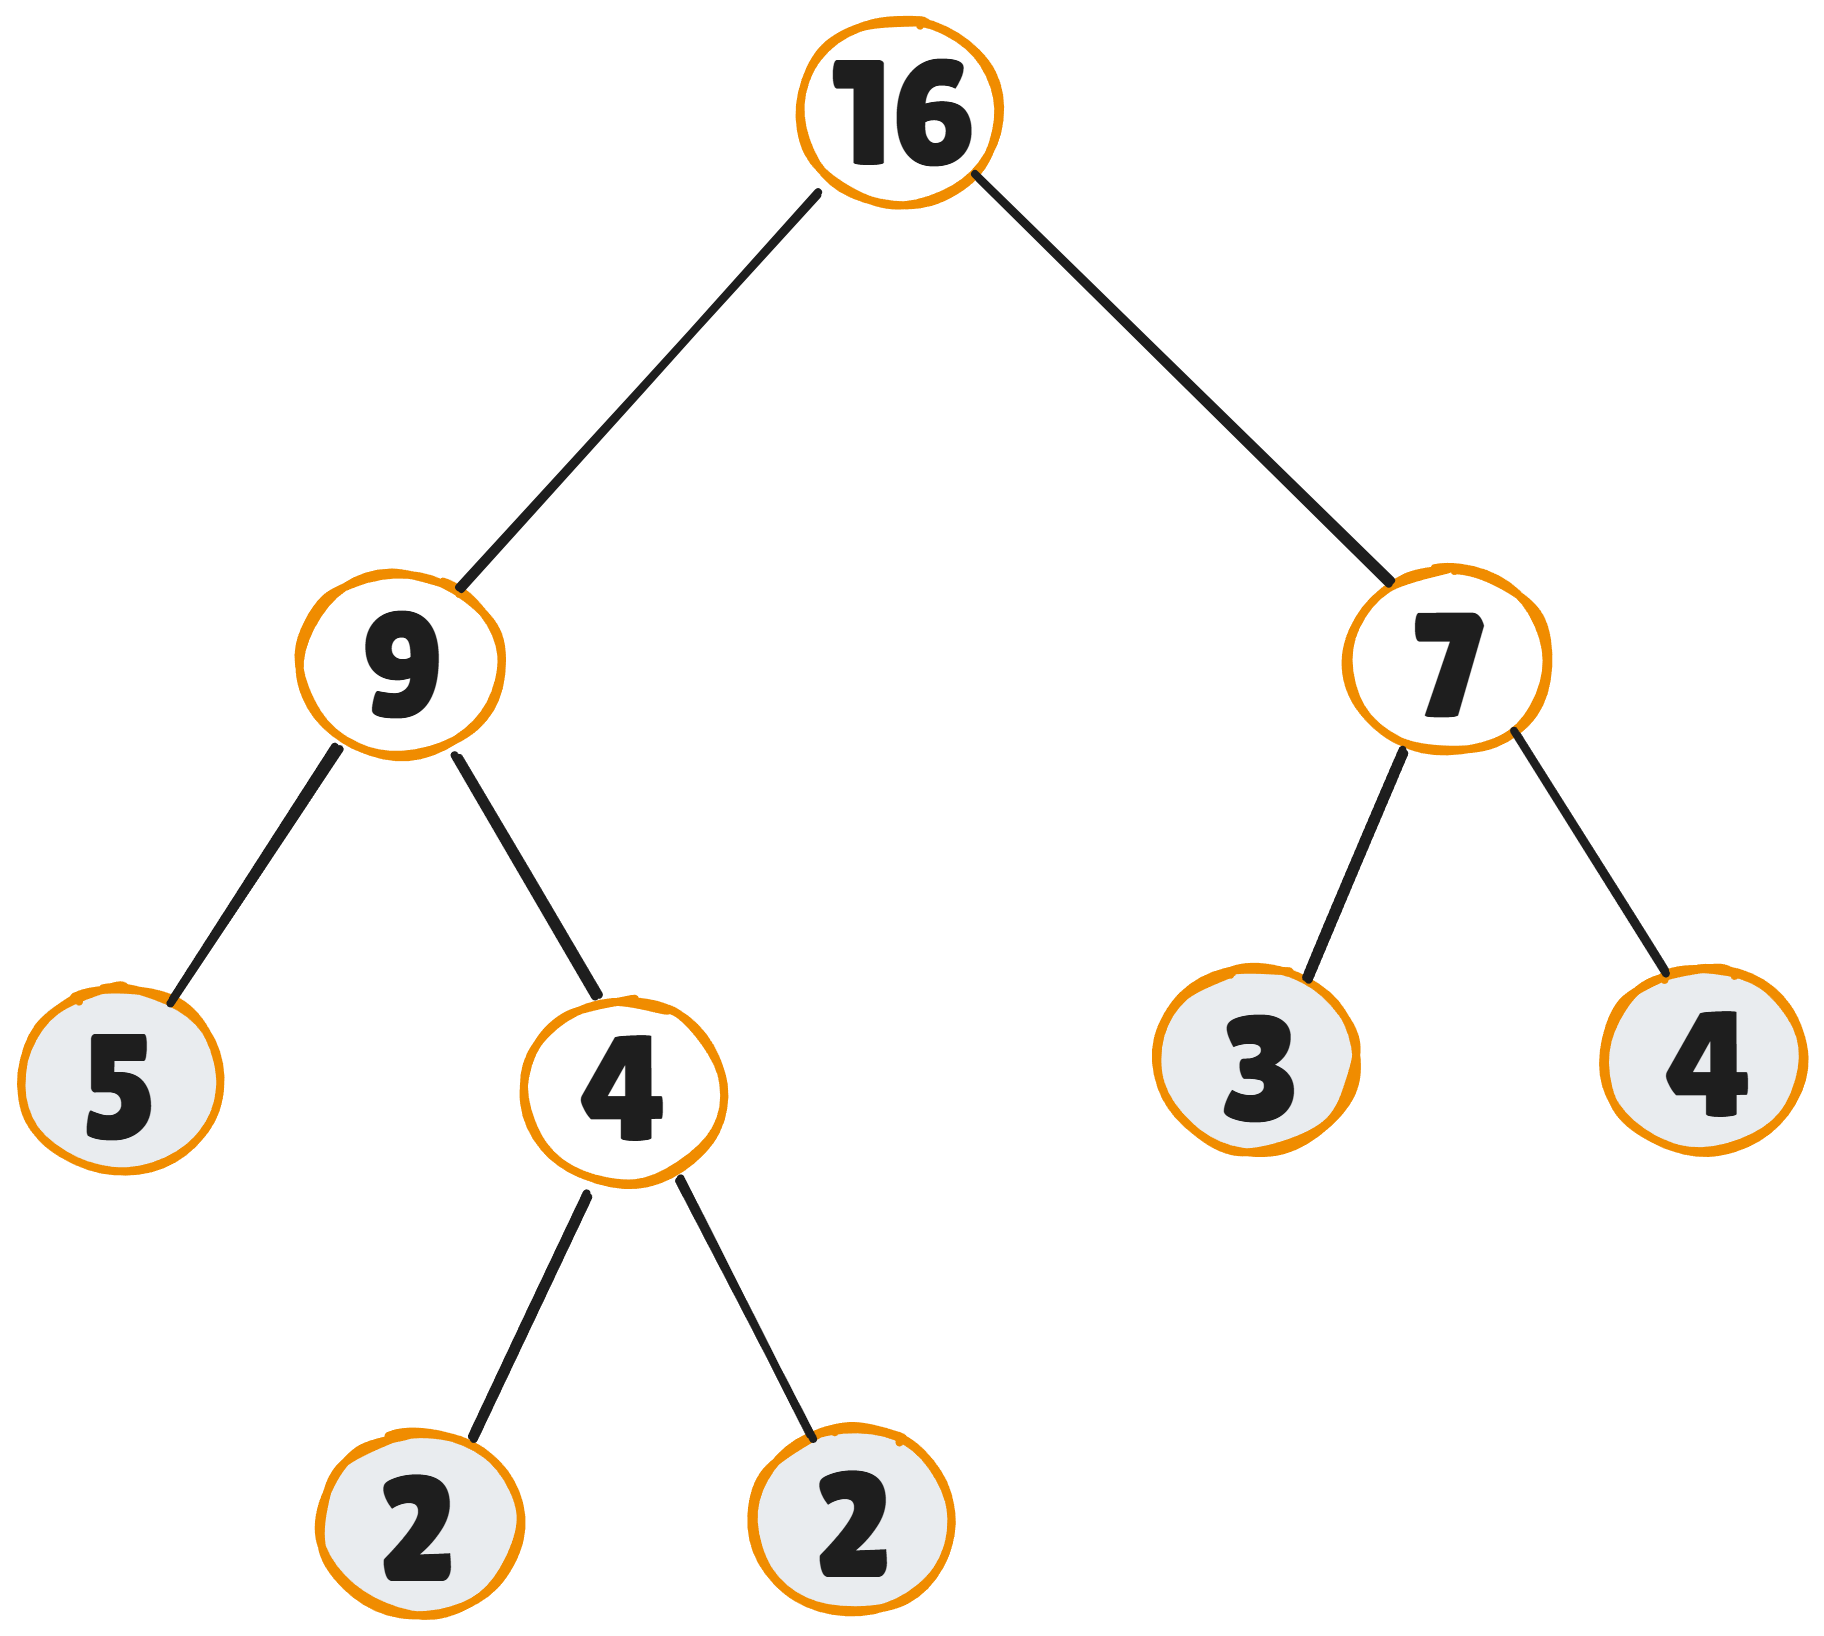
\includegraphics[width=0.4\linewidth]{img/ht3.png}
    \label{fig:enter-label}
\end{figure}

\end{bloco}
\end{frame}

\begin{frame}
\begin{bloco}[Revisitando a Árvore de Huffman]

\begin{itemize}
    \item Portanto, o algoritmo da Árvore de Huffman gera um custo ótimo para o problema. 
    \pause
    \item Aplicação: Desejamos multiplicar $n$ polinômios, e cada vez tomamos dois com menor grau possível, e resolvemos em $O((g_1 + g_2)\log(\max(g_1, g_2)))$, portanto, podemos multiplicar tudo em $O(\sum\limits_i g_i \log(\max\limits_i g_i)\log(n))$.
\end{itemize}

\end{bloco}
\end{frame}

\begin{frame}
\begin{bloco}[\textcolor{green}{password2} (\href{https://www.infoarena.ro/problema/password2}{infoarena})]

Dada uma senha secreta de comprimento $N$ composta pelas primeiras $S$ letras do alfabeto, você pode fazer consultas propondo cadeias de comprimento $N$. Para cada uma, recebe o comprimento do maior \textbf{prefixo} que aparece como \textbf{subsequência} na senha. Deve encontrar a senha com um máximo de $50000$ consultas.

\end{bloco}
\end{frame}

\begin{frame}
\begin{bloco}[\textcolor{green}{password2} (\href{https://www.infoarena.ro/problema/password2}{infoarena})]

\textbf{Idea:} realizar $S$ consultas para cada letra, depois podemos unir da seguinte forma:

\begin{itemize}
    \item Sejam as sequências $u_1, u_2, \dots, u_n$ e $v_1, v_2, ..., v_m$.
    \item Para cada $i$, desde $1$ até $n$, tentar colocar $u_i$ antes ou depois dos primeiros $j$ de $v$, note
    que tanto o índice $i$ (acerto) quanto o $j$ (erro) aumentam, portanto, pode ser realizado em $n + m$ consultas.
\end{itemize}

\end{bloco}
\end{frame}

\begin{frame}
\begin{bloco}[\textcolor{green}{password2} (\href{https://www.infoarena.ro/problema/password2}{infoarena})]

\begin{figure}
    \centering
    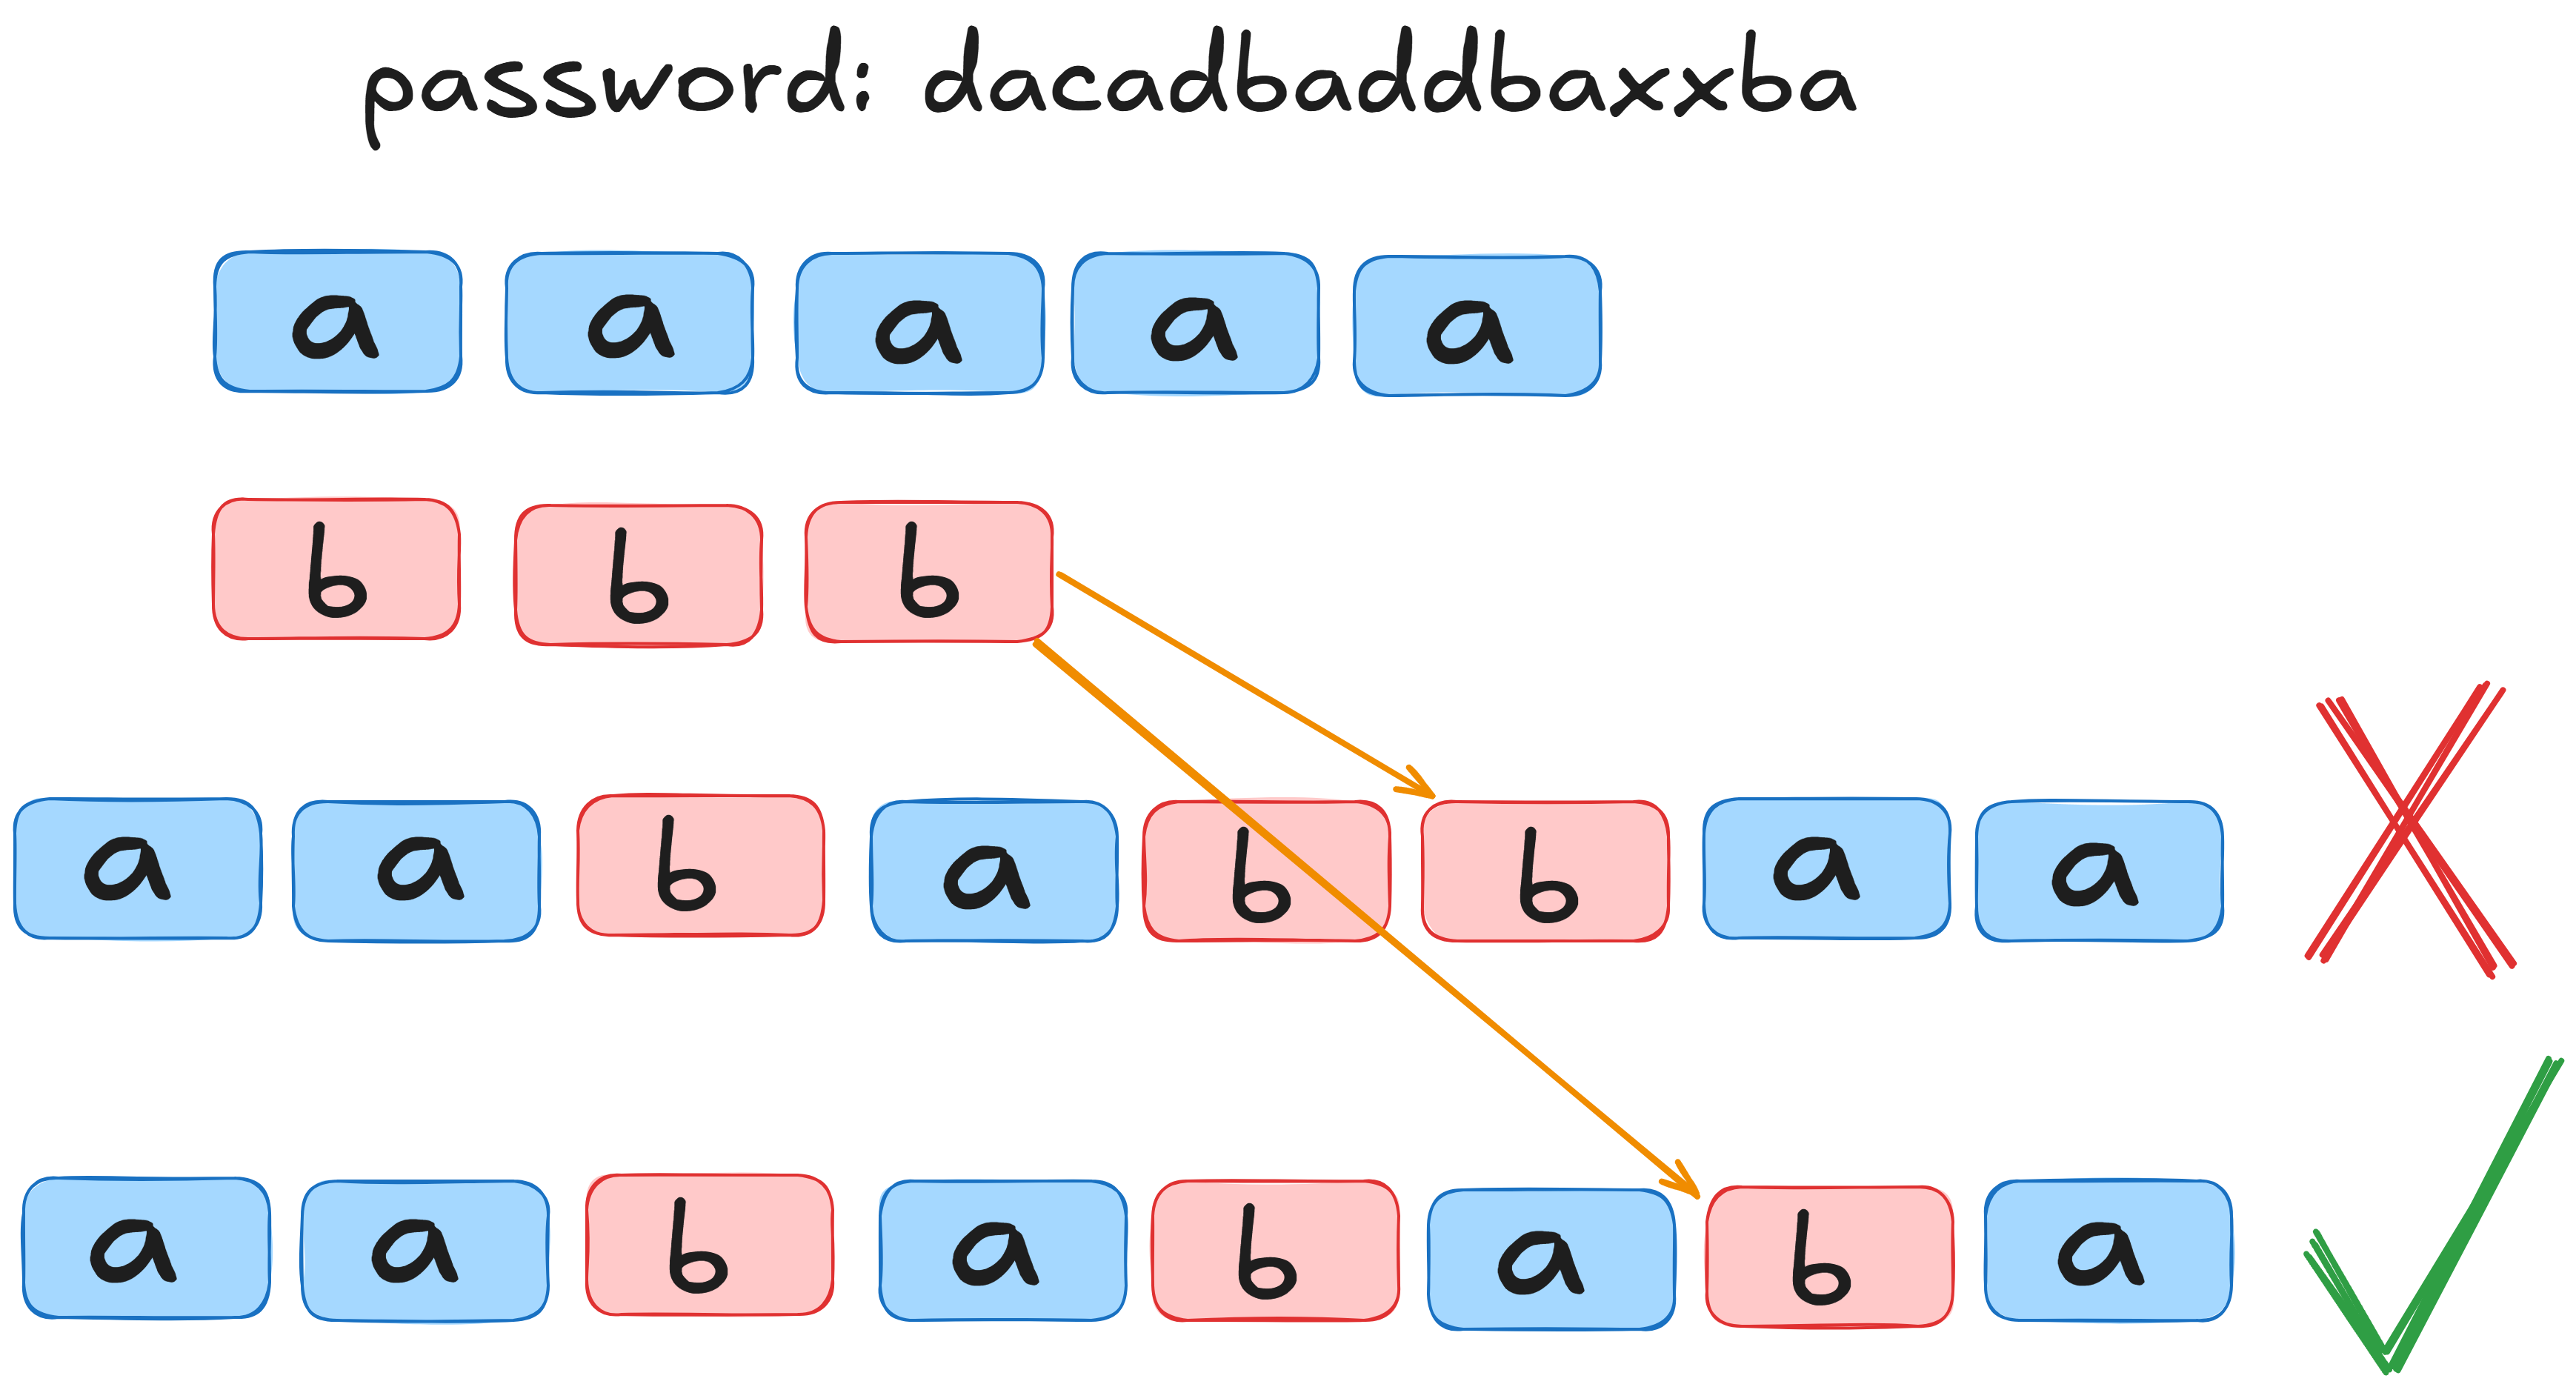
\includegraphics[width=0.8\linewidth]{img/select.png}
    \caption{União de duas sequências em ''dacadbaddbaxxba"}
    \label{fig:enter-label}
\end{figure}

\end{bloco}
\end{frame}

\begin{frame}
\begin{bloco}[\textcolor{green}{password2} (\href{https://www.infoarena.ro/problema/password2}{infoarena})]

\textbf{Idea:} realizar $S$ consultas para cada letra, depois podemos unir da seguinte forma:

\begin{itemize}
    \item Sejam as sequências $u_1, u_2, \dots, u_n$ e $v_1, v_2, ..., v_m$.
    \item Para cada $i$, desde $1$ até $n$, tentar colocar $u_i$ antes ou depois dos primeiros $j$ de $v$, note
    que tanto o índice $i$ (acerto) quanto o $j$ (erro) aumentam, portanto, pode ser realizado em $n + m$ consultas.
    \item resolvemos com o algoritmo da Árvore de Huffman, portanto, gastamos no máximo $S + N\log S$ consultas.
\end{itemize}

\end{bloco}
\end{frame}

\begin{frame}{Argumento Estrutural e de Troca}
\begin{definicao}
\begin{itemize}
    \item {\bfseries Arg. Estrutural}: Prova que qualquer solução ótima deve ter certa estrutura. Ex: Existe uma Árvore de Huffman, tal que nós com menor peso são irmãos.
    \item {\bfseries Arg. Troca}: Comparamos a solução do algoritmo com uma ótima e mostramos que trocar partes melhora ou não piora.
\end{itemize}
\end{definicao}
\end{frame}

\begin{frame}
\begin{bloco}[\textcolor{black}{POI 2007 Weights} (\href{https://szkopul.edu.pl/problemset/problem/h_QPStxSmfEHuL2h_I5Qpa29/site/?key=statement}{szkopul})]

Temos $n$ contêineres com capacidades $c_1, c_2, \dots, c_n$ e $m$ pesos com massas $w_1, w_2, \dots, w_m$. Cada contêiner pode conter qualquer número de pesos, desde que a soma de suas massas não exceda sua capacidade. Além disso, para todo par $i, j$, vale que $w_i \mid w_j$ ou $w_j \mid w_i$. Deseja-se encontrar a quantidade máxima de pesos que podem ser colocados respeitando estas condições.

\end{bloco}
\end{frame}

\begin{frame}
\begin{bloco}[\textcolor{black}{POI 2007 Weights} (\href{https://szkopul.edu.pl/problemset/problem/h_QPStxSmfEHuL2h_I5Qpa29/site/?key=statement}{szkopul})]

\textbf{Idea:} 

\begin{itemize}
    \item Podemos usar \textbf{busca binária} sobre a quantidade de pesos a colocar -- testamos se é possível com os $k$ menores pesos --.
    \pause
    \item Seja $S$ um conjunto de pesos que pode ser colocado completamente nos contêineres sem exceder suas capacidades, e seja $m_{max}$ a massa do peso mais pesado em $S$. Denotamos por $C(S)$ o conjunto de todas as configurações válidas para $S$.
\end{itemize}
\end{bloco}
\end{frame}

\begin{frame}
\begin{bloco}[\textcolor{black}{POI 2007 Weights} (\href{https://szkopul.edu.pl/problemset/problem/h_QPStxSmfEHuL2h_I5Qpa29/site/?key=statement}{szkopul})]

\textbf{Idea:} 

\begin{itemize}
    \item \textbf{Argumento Estrutural:} 
    Para qualquer contêiner $t$ com capacidade $w_t \geq m_{\max}$, existe uma configuração válida $\mathcal{C}^* \in C(S)$ onde o peso $m_{\max}$ está colocado em $t$.
\end{itemize}
\end{bloco}
\end{frame}

\begin{frame}
\begin{bloco}[\textcolor{black}{POI 2007 Weights} (\href{https://szkopul.edu.pl/problemset/problem/h_QPStxSmfEHuL2h_I5Qpa29/site/?key=statement}{szkopul})]

\textbf{Prova:} 

Seja uma configuração qualquer e vejamos que podemos colocar $m_{max}$ em $j$.   

\begin{itemize}
    \item Se a soma dos pesos no contêiner $j$ for menor ou igual ao peso máximo, podemos trocá-los sem nenhum problema. 
    \pause
    \item Caso contrário, ordenamos o contêiner $j$, do maior para o menor $w^{'}_1, w^{'}_2, ..., w^{'}_m$, seja $k$ tal que \(\sum\limits_{i=1}^k w^{'}_i \le m_{max} < \sum\limits_{i=1}^{k+1} w^{'}_i\), vale $\sum\limits_{i=1}^k w^{'}_i = m_{max}$ 
\end{itemize}
\end{bloco}

\end{frame}

\begin{frame}
\begin{bloco}[\textcolor{black}{POI 2007 Weights} (\href{https://szkopul.edu.pl/problemset/problem/h_QPStxSmfEHuL2h_I5Qpa29/site/?key=statement}{szkopul})]

    
\textbf{dica:} Note que $w^{'}_1 \vert m_{max}$, e em geral $w^{'}_{r + 1} \vert (m_{max} - \sum\limits_{i=1}^r w^{'}_i)$, para todo $r \le k$.
    
\end{bloco}

\end{frame}


\begin{frame}
\begin{bloco}[\textcolor{blue}{Moedas} (Olimpíada Polonesa Júnior)]
São dadas $n$ pilhas de moedas. Cada pilha contém exatamente duas moedas. Conhece-se o valor de cada uma das $2n$ moedas. Pode-se selecionar no máximo $k$ moedas, com a seguinte restrição: 

\begin{itemize}
    \item \textbf{Se escolher a moeda inferior de uma pilha, também deve escolher a superior da mesma pilha.}
\end{itemize}

Determine o valor total máximo que pode ser obtido ao selecionar as moedas

\end{bloco}
\end{frame}

\begin{frame}
\begin{bloco}[\textcolor{blue}{Moedas} (Olimpíada Polonesa Júnior)]

\textbf{Idea:}
\begin{itemize}
    \item Há dois tipos de pilhas, as que têm o valor máximo no topo, e as que não têm.
    \pause
    \item \textbf{Argumento de troca:} Se só há pilhas do tipo 1. Existe uma solução ótima que respeita a condição de ordem na escolha. (\textbf{dica:} Nunca é ótimo tomar a ficha de baixo antes que a de cima)
\end{itemize}

\end{bloco}
\end{frame}

\begin{frame}
\begin{bloco}[\textcolor{blue}{Moedas} (Olimpíada Polonesa Júnior)]

\begin{itemize}
    \item \textbf{Argumento Estrutural:} Se só há fichas do tipo 2. Existe uma solução que só toma no máximo uma ficha de cima sem sua ficha de baixo.\\
    \pause
    \textbf{Prova:} Sejam as pilhas $p_1 = (a_1, b_1)$ e $p_2 = (a_2, b_2)$, tal que $a_1 < b_1$ e $a_2 < b_2$, sem perda de generalidade $a_1 \le a_2$. Então

\[
    a_1 + a_2 ~(\text{tomar o topo de ambas}) < 
\]
\[
    a_2 + b_2 ~(\text{tomar só uma})
\]

    Duas pilhas não podem ser tomadas parcialmente.

\end{itemize}

\end{bloco}
\end{frame}

\begin{frame}
\begin{bloco}[\textcolor{blue}{Moedas} (Olimpíada Polonesa Júnior)]

\begin{itemize}
    
    \item Se tomamos $k_1$ fichas de pilhas do tipo 1, estas sempre podem ser as $k_1$ fichas maiores, se tomamos $k_2$ fichas de pilhas do tipo 2, se for uma quantidade par, tomamos as $k_2 / 2$ pilhas com valor total maior, caso contrário tomamos a maior ficha de topo não escolhida, ou tomamos a próxima maior pilha e removemos a menor ficha de baixo escolhida.   
    
\end{itemize}

\end{bloco}
\end{frame}

\begin{frame}
\begin{bloco}[\textcolor{blue}{Moedas} (Olimpíada Polonesa Júnior) ]

\begin{figure}
    \centering
    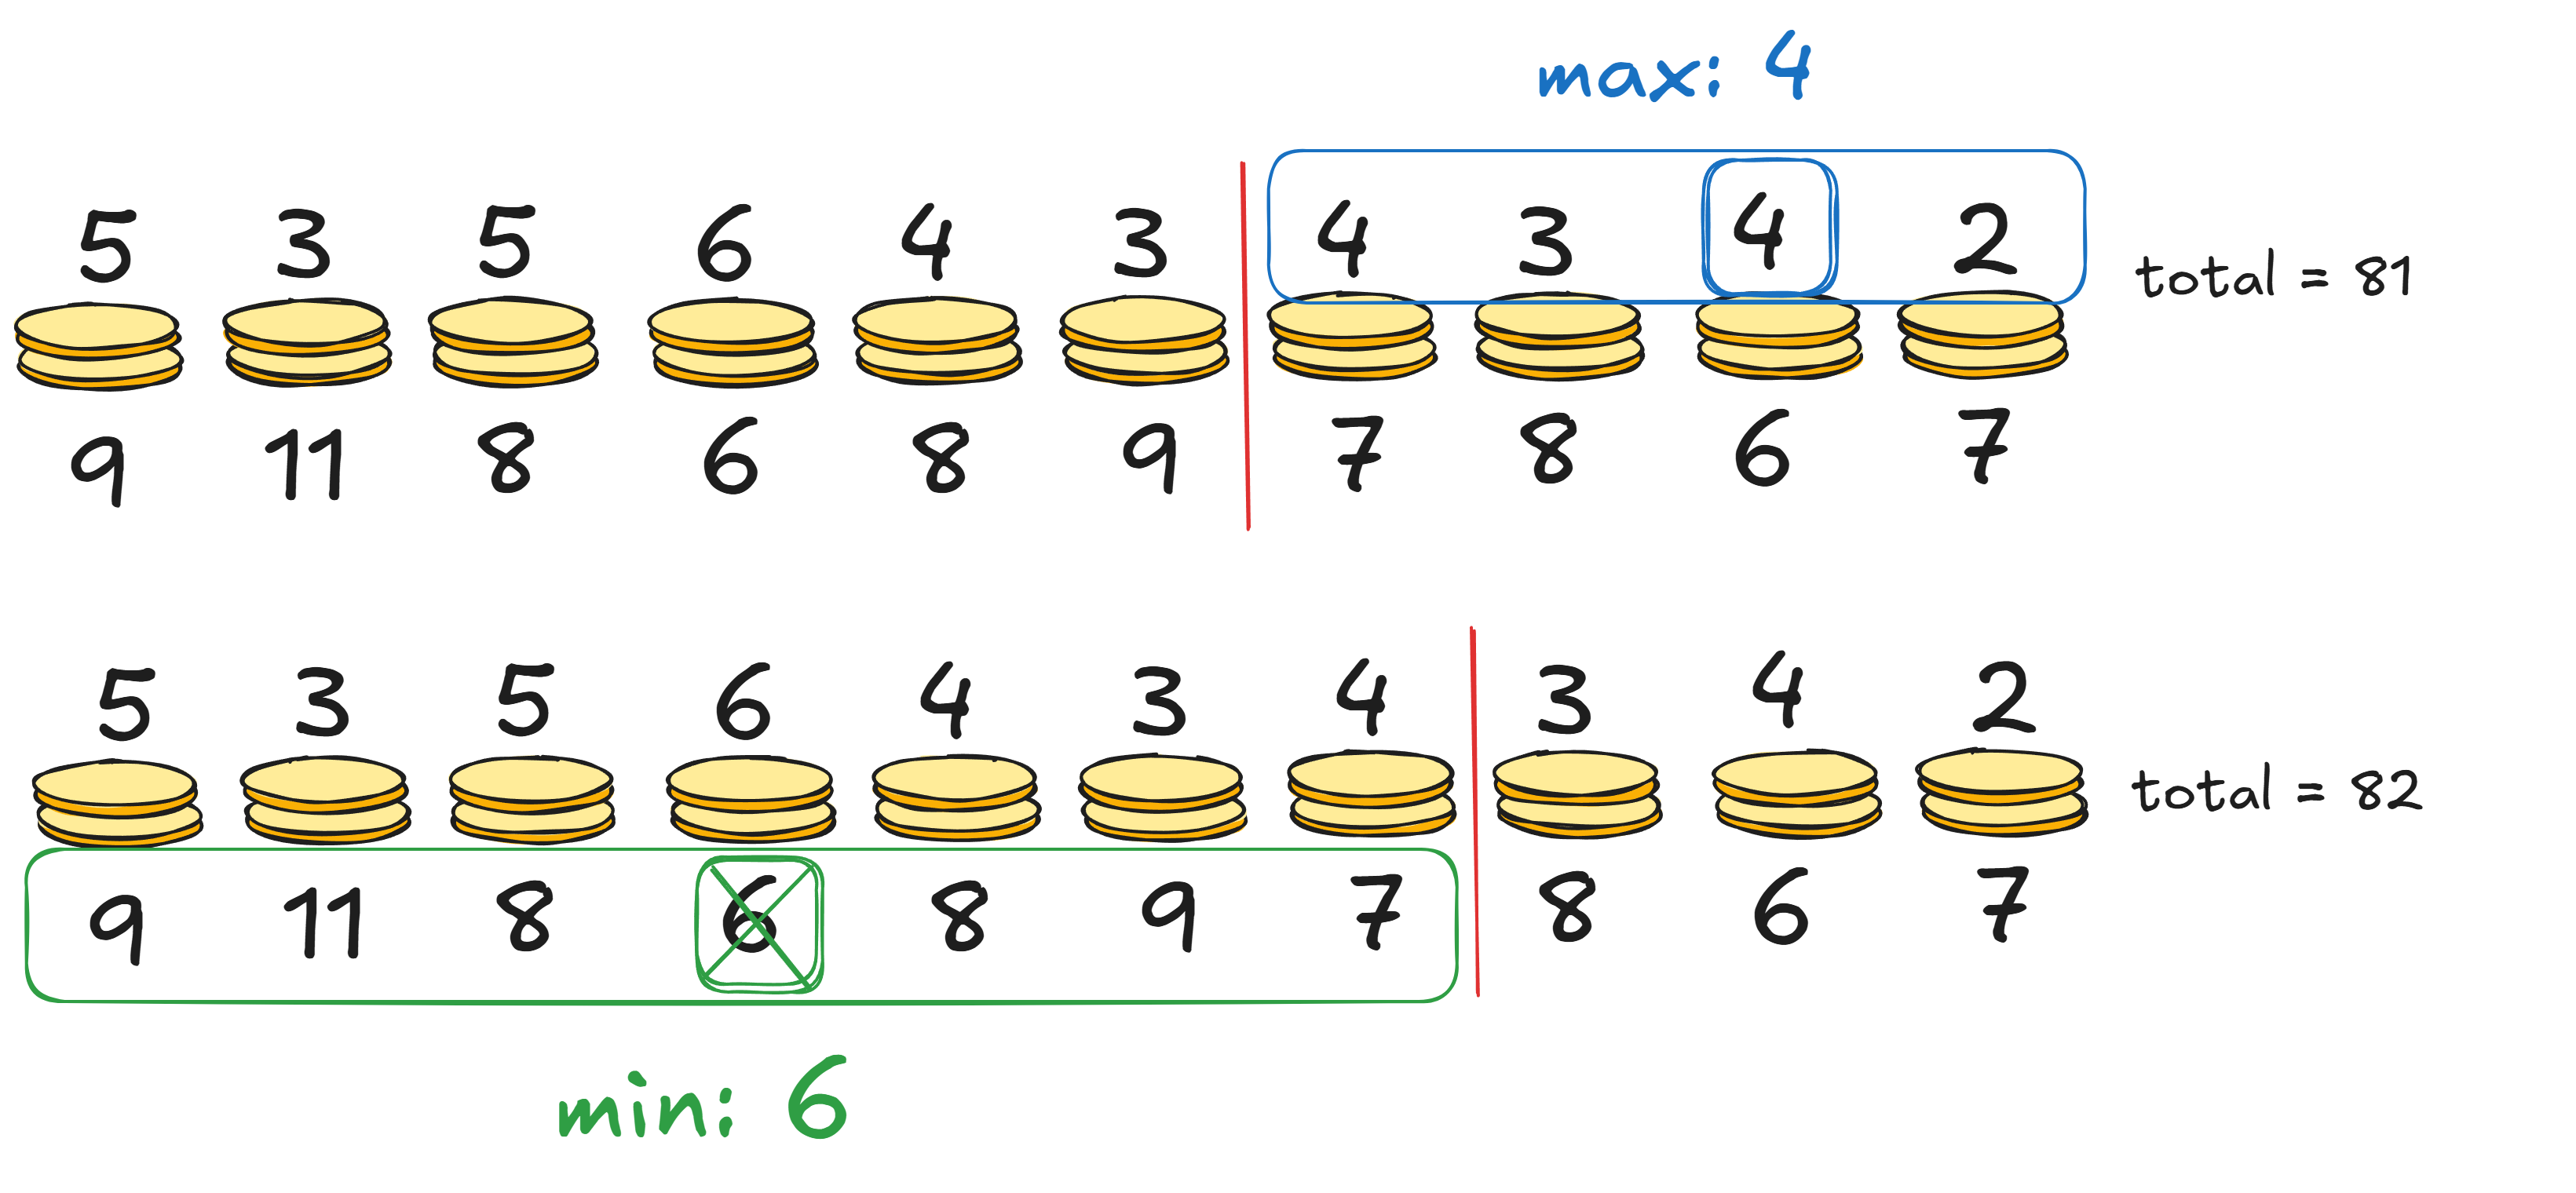
\includegraphics[width=0.97\linewidth]{img/coins-greedy.png}
    \caption{Escolha de $k=7$ fichas de pilhas do tipo 2.}
    \label{fig:enter-label}
\end{figure}

\end{bloco}
\end{frame}

\begin{frame}

\centering
\Large Obrigado.

\end{frame}
\end{document}